\begin{enumerate}
	\item $\phantom{X}$
	
	\fbox{
	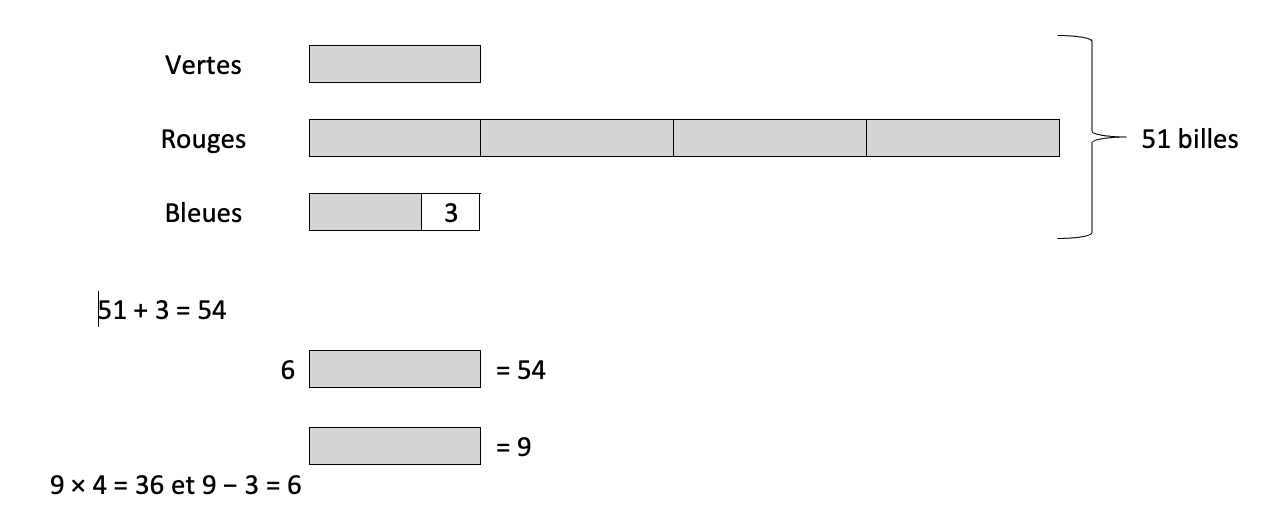
\includegraphics[width=\linewidth]{images/2022-g1-ex3-corr-img1.png}
	}
	
	\medskip
	Il y a 9 billes vertes, 36 billes rouges et 6 billes bleues.
	
	\item 
	\begin{enumerate}
		\item Soit $r$ le nombre de billes rouges et $b$ le nombre de billes bleues.\\
		On peut noter : $r=4\times v$ et $b=v-3$.
		
		\item On obtient l'équation suivante : \\
		$v+4\times v+v-3=51$\\
		$6v-3=51$ (on ajoute 3 aux deux membres)\\
		$6v=54$ (on divise par 6 les deux membres)\\
		$v=9$
		
		\medskip
		Donc : $r=4\times9=36$ et $b=v-3=9-3=6$. 
	\end{enumerate}
\end{enumerate}